\documentclass[a4paper,12pt]{report}
\usepackage[utf8]{inputenc}
\usepackage[left=1.25in, right=1.25in]{geometry}
\usepackage{graphicx}
\usepackage{titlesec}
\usepackage{hyperref}
\usepackage{adjustbox}
\usepackage{epigraph}
\usepackage{listings}
\usepackage{xcolor}
\usepackage{float}
\usepackage[super, numbers, square]{natbib}

\definecolor{lightgray}{rgb}{0.97,0.97,0.97}
\definecolor{darkgreen}{rgb}{0.2,0.5,0.2}
\definecolor{darkred}{rgb}{0.64,0.09,0.09}
\lstset{ 
	backgroundcolor=\color{lightgray},
	basicstyle=\fontsize{8}{12}\ttfamily,
	breakatwhitespace=false,
	breaklines=true,
	captionpos=b,,
	escapeinside={\%*}{*)},
	extendedchars=true,
	commentstyle=\color{blue},
	frame=single,
	keepspaces=true,
	keywordstyle=\color{darkred},
	language=SQL,
	morekeywords={GROUP\_CONCAT, FILTER, OPTIONAL, BIND, BOUND},
	deletekeywords={KEY,YEAR,ELSE},
	numbers=none,
	rulecolor=\color{gray},
	showspaces=false,
	showstringspaces=false,
	showtabs=false,
	stepnumber=2,
	stringstyle=\color{darkgreen},
	tabsize=2
}
\renewcommand{\bibname}{References}
\graphicspath{ {images/} }
\setlength\epigraphwidth{0.7\textwidth}
\title{Developing a virtual assistant for answering music related questions}
\author{Claudio SCALZO \\ (\href{mailto:scalzo@eurecom.fr}{scalzo@eurecom.fr}) \and Luca LOMBARDO \\ (\href{mailto:lombardo@eurecom.fr}{lombardo@eurecom.fr}) }
\date{\textit{Professor}: Raphaël Troncy\\\textit{Supervisors}: Pasquale Lisena~~-~~Thibault Ehrhart}

\begin{document}
\maketitle
\tableofcontents

\chapter{Introduction}
	\section{Why a virtual assistant?}
	In these years we're assisting to a huge development of virtual assistants, mainly in two different shapes: vocal assistant and chat bots. Usually, each of the tasks that the user asks to the virtual assistant are tasks that can be done in other ways; we can think about a user asking for directions to \textit{Siri} or a user who tells his \textit{Google Assistant} to schedule an appointment in his calendar. Each of these are tasks that can be done without the help of an assistant! So, why they are becoming so popular? The reason is of course related to the ease of use. There are tasks which are, even if easy, boring or annoying to do, and we can take as example the scheduling of an appointment: we can unlock the phone, open an app, write the name of the appointment, select the start date and the end date, select the reminder scheduling, select the option to keep it private or make it public, and select other options depending on which calendar app we're using. Easy of course, but way more complicated than saying: \textit{"Hey Google, set me an appointment with Luca for tomorrow afternoon at 5pm, and please remind me 2 hours before"}.\\\\
	Having said that, the reason behind the development of our virtual assistant should be clear: simplify the user's life when he wants to access some informations about classical music.
	
	\section{Scope of the project}
	Our project puts down its root into \textit{DOREMUS}\cite{doremus}, a classical music knowledge graph, mainly composed by an ontology of 64 classes and 250 properties, and a set of 17 vocabularies. The informations contained inside \textit{DOREMUS} can be accessed thanks to a SPARQL endpoint, that lets users write queries to retrieve the set of data they want to achieve.\\\\
	Our project starts from this difficulty: how many people know SPARQL? And inside the set of people who know it, how many problems can rise using the SPARQL language? Using the right properties, checking the exact domain and ranges for each property and other annoying problems just to obtain simple results. Our bot faces this issue, making simple to obtain the most common informations the users want.
	
	\section{Aim and expected results}
	The real aim of the virtual assistant so, is to make simpler the use of the \textit{DOREMUS} knowledge graph and the retrieval of its data. But which will be our, concrete, final results? First of all, the shape of the virtual assistant is originally a chat bot. The queries are textually written and the responses are visually seen on the display of each device running a client with the bot installed. This, of course, is not the only shape the bot can have. It can be a vocal assistant, and the query can be done by voice. In each of the cases, the bot will extract the informations from the \textit{DOREMUS} knowledge graph using SPARQL queries, answering to the user's requests and without letting them know a single detail about the SPARQL query that is using or other technical details. It will also help the user to make a more detailed and precise query (guiding him with some questions), and will correct the users sentences when he does some typos or when he's wrong in writing some precise words (like artist names, instruments or musical genres).

\chapter{Natural Language Understanding}
	\section{What is NLU?}
	Natural language understanding \textit{(NLU)} is an artificial intelligence technique that deals with the automatic treatment of informations provided in a given natural language. It puts its roots into the first works by Daniel Bobrow\cite{bobrow} in 1964 and the \textit{ELIZA}\cite{eliza} project in 1965, by Joseph Weizenbaum. The interest in \textit{NLU} has become in the years bigger and bigger, and after some interesting works like the one of William Woods\cite{woods}, who introduced the \textit{ATN (Augmented Transition Network)} in the natural language processing field, the research focused (in the 70s and 80s) in using machine learning techniques to fulfill natural language processing tasks.
	\section{NLP, NLU and NLG}
	\textit{Natural Language Processing (NLP)}, \textit{Natural Language Understanding (NLU)} and \textit{Natural Languange Generation (NLG)} are similar terms that doesn't share the same meaning. 
	\begin{figure}[H]
		\centering
		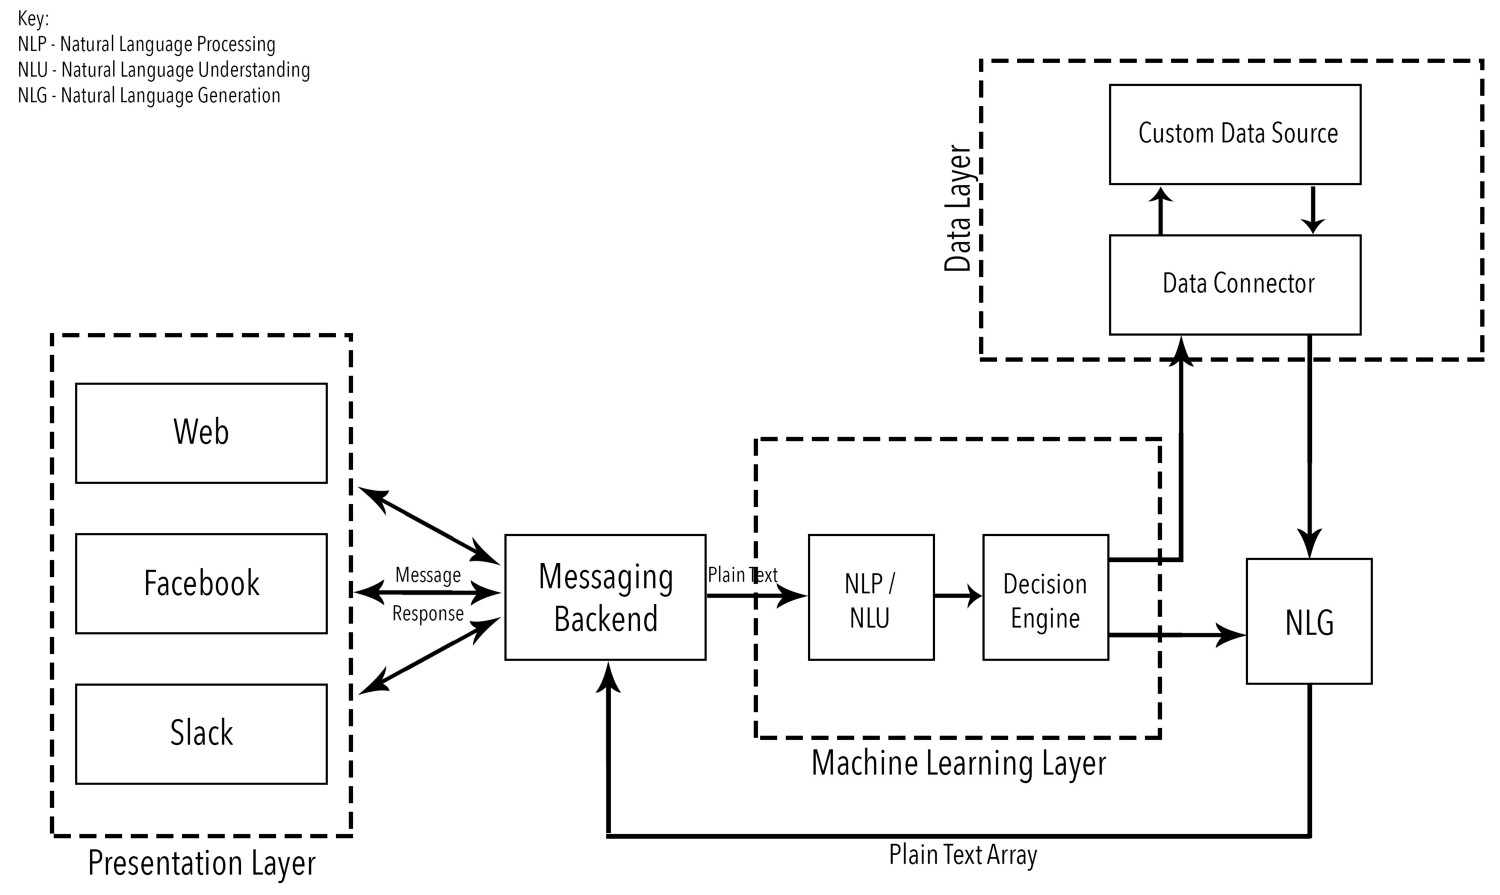
\includegraphics[scale=0.2]{nlschema}
		\caption{NLP, NLU, NLG and how Chatbots work.\cite{nlpnlunlg}}
	\end{figure}
	\begin{itemize}
	\item \textit{NLP} is the biggest set between the three, because it's a term which indicates the capability of a software to ingest an input sentence, split it in pieces (entities), understand the entities and their relationship, and give the answer to the user.
	
	\item \textit{NLU} is a subset of \textit{NLP}. It deals with understanding a natural language input (totally or partially unstructured) and convert it into a structured form that the machine can process and understand. Is a small yet critical task to achieve.
	
	\item \textit{NLG} can be seen as the dual phase of \textit{NLU}: turning structured data into natural language, to give the user the answer he wants.
	\end{itemize}
	
	\section{How machine learning can help NLU?}
	\subsection{Attention-Based RNN model for joint intent detection and slot-filling}
	One interesting work that can help in understanding the strong relationship between natural language understanding and machine learning, can be the one by Bing Liu and Ian Lane\cite{rnn}. Intent detection and slot-filling are indeed crucial parts of NLU: intent detection can be seen as a classification problem were, given a set of words (the sentence), the algorithm is capable to classify that sentence and give it a label which will correspond to one of the intents that the machine is able to recognize. Slot-filling can be just seen as a sequence labeling task. For what regards the intent detection phase, the classification problem can be faced by popular machine learning algorithms like \textit{Neural Networks (NNs)} or \textit{Support Vector Machines (SVMs)}; instead, for the slot-filling sequence labeling task, useful tools can be \textit{Markov models (MEMMs)} and \textit{Conditional Random Fields (CRFs)}.\\\\
	Is fundamental in this case, to understand the concept of alignment:
	\begin{itemize}
		\item Alignment is present when the output of the encoder is the same input given to the decoder. Is the case of slot-filling, where the entire set of entities is aligned (when processed with the encoder, can be directly given to the decoder).
		
		\item Alignment is not present when the output of the encoder can't be directly given in input to the decoder. An additional processing phase is needed before feeding the decoder with the informations it needs as input. is the case of the intent detection, where the decoder needs the information of all the words to detect the intent.
	\end{itemize}
	In both intent detection and slot-filling tasks, \textit{RNNs (Recurrent Neural Networks)} can be (and have been) applied:\\\\
	In the case of slot-filling, the input-output sequence is explicitly aligned, with a "slot" to fill for each single information extracted from the sentence. The models used in the years, in this case, have the aim to maximize the likelihood:
	\begin{equation}
	\arg \max_{\theta} \prod_{t=1}^{T} P(y\textsubscript{t}|y\textsubscript{1}\textsuperscript{t-1},x;\theta)
	\end{equation}
	Another structure exploiting RNNs can be instead the RNN Encoder-Decoder framework: in this case the input-output sequence is not aligned, and this structure is of course better for an intent detection task. In this case, the encoder and the decoder are separated entities: the encoder reads a sequence of inputs into a context vector \textit{c}, which is used from the decoder as source of informations for fulfilling its task. The probability of the output sequence of the decoder is:
	\begin{equation}
	P(y) = \prod_{t=1}^{T} P(y\textsubscript{t}|y\textsubscript{1}\textsuperscript{t-1},c)
	\end{equation}
	The work conducted by Liu and Lane aims to propose two different alternatives to be able to work well in joint intent detection and slot-filling tasks.
	\begin{figure}[H]
		\centering
		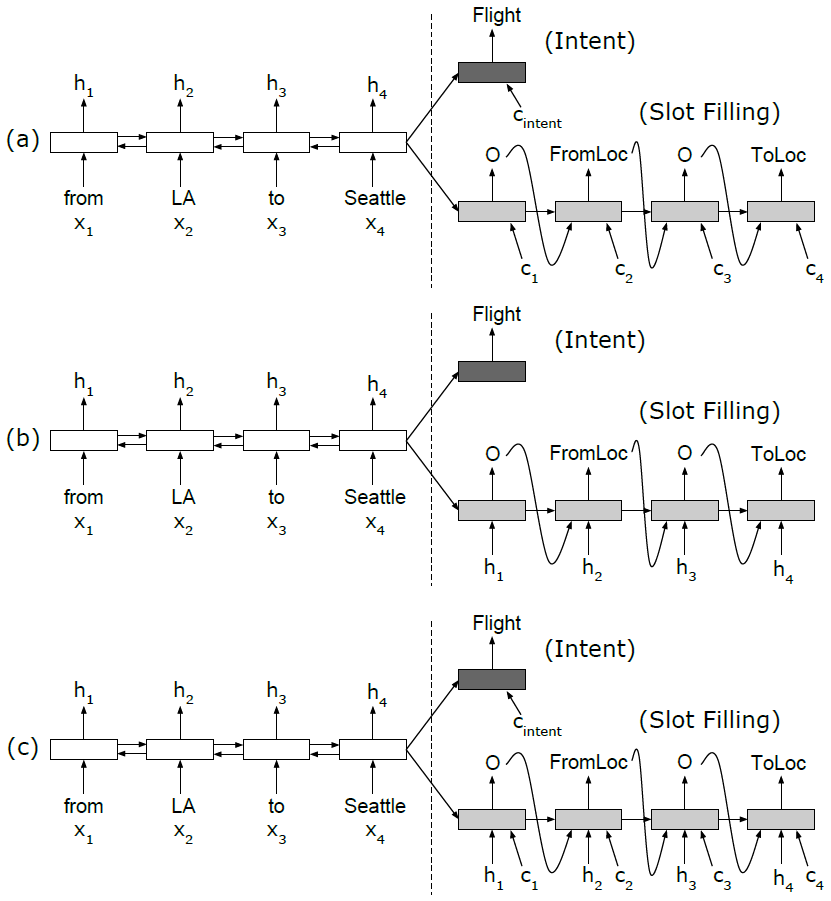
\includegraphics[scale=0.4]{alt1}
		\caption{The three alternatives using the Encoder/Decoder model.}
	\end{figure}
	In this case, as the figure shows, the encoder and the decoder phase are separated. In the encoder phase we can find the \textit{bidirectional RNNs}: each of them produces an hidden "forward" state \textit{fh\textsubscript{i}} and an hidden "backward" state \textit{bh\textsubscript{i}}. The output of the last \textit{RNN} is used for the intent detection and to initialize the decoder \textit{RNN} state.\\\\
	In the subfigure \textit{(a)}, we can find an example of non-aligned inputs. Indeed, the input given to the decoder phase is the context vector \textit{c}, produced by a weighted sum of all components of the \textit{h} vector produced by the encoder phase.\\
	In the subfigure \textit{(b)}, the inputs are aligned. The input vector of the decoder phase is just the \textit{h} array.\\
	The last subfigure \textit{(c)} shows a situation with aligned inputs and also the addition of attention. This is useful for the joint intent classification and slot-filling task: both the \textit{h} and the \textit{c} vectors are used in the decoder phase, that shows also an intent detection taking as input the output of the last \textit{RNN} and also the \textit{c} context vector.
	\begin{figure}[H]
		\centering
		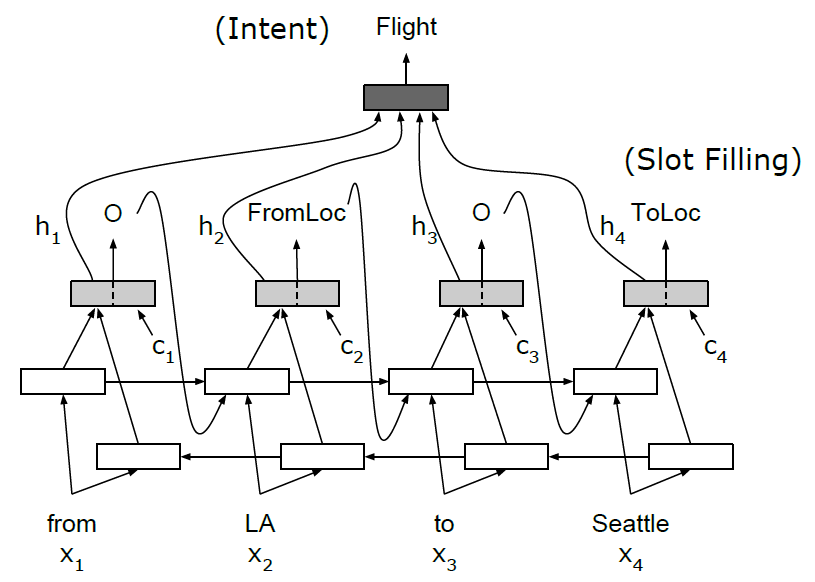
\includegraphics[scale=0.4]{alt2}
		\caption{Attention-based RNN model for joint intent detection
			and slot filling.}
	\end{figure}
	The attention-based model proposed by Liu and Lane shows a clear structure: each bidirectional \textit{RNN} produces a forward and a backward hidden state, useful for predicting the slot label (the core of the slot-filling task). At the same time, these outputs \textit{h\textsubscript{i}} are merged with the context vector \textit{c} to predict the final intent label.
	
	\subsection{A Unified Architecture for Natural Language Processing: Deep Neural Networks with Multitask Learning}
	One fundamental work in the Natural Language Processing worlds is the one by Collobert and Weston\cite{unified}. In their work, they propose a deep neural network that learns relevant features also with limited prior knowledge.\\\\
	The different tasks considered in the work are:
	\begin{itemize}
		\item Part-Of-Speech Tagging (POS): labeling each word with its role in the sentence (noun, adverb, verd, etc.).
		\item Chunking: labeling segments of sentences, with each word tagged as begin-chunk or inside-chunk.
		\item Named Entity Recognition (NER): labels elements in the sentence in categories (person, city, company, etc.).
		\item Semantic Role Labeling (SRL): gives a semantic role to a constituent of a sentence.
		\item Language Models: estimates the probability of the next word to be \textit{w} in a given word sequence.
		\item Semantically Related Word: understand if two words are semantically related (synonyms, holonymns, etc.).
	\end{itemize}
	\begin{figure}[H]
		\centering
		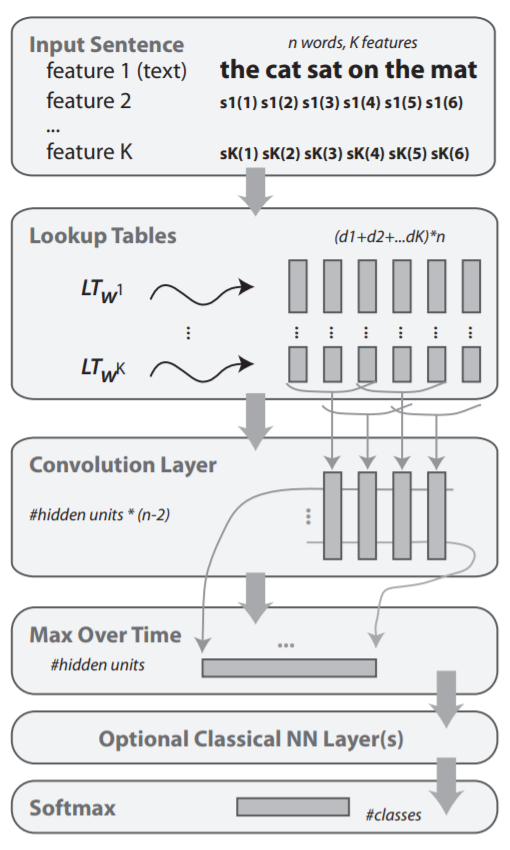
\includegraphics[scale=0.4]{unified}
		\caption{Deep Neural Networks for Natural Language Processing\cite{unified}.}
	\end{figure}
	In the proposed model, each word is considered as part of a given table:
	\begin{equation}
	LT_w(i) = W_i
	\end{equation}
	where the W term is the set of parameters to be learned. So, in the first layer of the network the input sequence is transformed into a set of vectors ${W_i}$.\\\\
	The output is then computed by the second layer, which performs convolutional operations:
	\begin{equation}
	o(t) = \sum_{j=1-t}^{n-t} L_j \cdot x_{t+j}
	\end{equation}
	where the \texttt{L} parameters are trained by back-propagation.\\\\
	Then, a layer follows the convolutional ones: it takes the most relevant features of the sentence feeding the output into a "\textit{Max}" Layer. It's important to notice that the output is of fixed length: this means that classical neural networks can be appended and trained for the labeling tasks.\\\\
	An important feature of the proposed model is the ability to perform multitask learning (MTL), in a deep joint training fashion. The network automatically learns features for each task in the various layers of the architecture: the deepest layers (with lookup-tables) learns the features for each word in the dictionary, so using them in common for related tasks (during training) can improve the overall generalization performance. In the work proposed by Collobert and Weston indeed, training is done in a stochastic fashion (keeping in mind that the labeled data for each task can be different, also coming from different datasets):
	\begin{enumerate}
		\item Take the next task.
		\item Select a training example for this specific task.
		\item Train the neural network (updating weights) using the gradient with respect to the example.
		\item Restart from point 1.
	\end{enumerate}

	\section{State of art: famous and most used tools}
	\begin{itemize}
		\item \textbf{Wit.ai}\cite{witai}\\
		Facebook owned, is one of the most complete solutions for natural language processing. It supports 50 languages, it’s free.
		
		Pros:
		\begin{itemize}
			\item Supports machine learning to learn alternative phrases.
			\item UI to work with intent and entities.
			\item Developer view with conversation flows, context variables, branching logic.
			\item Supports "roles" in entities (e.g. \texttt{fromLocation(Nice)} to \texttt{toLocation(Turin)}).
		\end{itemize}
		
		Cons:
		\begin{itemize}
			\item No "required field" option (slot-filling)
		\end{itemize}	

		\item \textbf{Snips}\cite{snips}\\
		An open source alternative to the most popular NLU systems.
		
		Pros:
		\begin{itemize}
			\item Fully runs on device.
			\item Heavily exploits machine learning (especially CRF).
			\item Privacy by design.
			\item Precise performance metrics .
			\item Open source (\textit{\href{https://github.com/snipsco}{https://github.com/snipsco}}).
			\item Integrated Automatic Speech Recognition.
		\end{itemize}
		
		Cons:
		\begin{itemize}
			\item Doesn't support a big set of languages.
		\end{itemize}
	
		\item \textbf{IBM Watson}\cite{watson}\\
		\textit{"The first choice as a bot-building platform for 61\% of businesses".}\\
		It supports Node, Java, Python, iOS and Unity SDK. Free and Premium plans. It’s heavy but powerful.
		
		\item \textbf{Amazon Lex}\cite{lex}\\
		It powers \textit{Alexa}. SDKs for popular platforms.\\
		You pay only for what you use. No demo, no open-source.
		
		\item \textbf{Microsoft LUIS}\cite{luis}\\
		Supports and heavily uses machine learning. Composite entities (e.g. \textit{"2-adults first class flight ticket"}). Rich metrics of performances evaluation of the assistant.
		
		\item \textbf{Recast.ai}\cite{recast}\\
		SAP-owned. \textit{"Free"} and \textit{"Company"} accounts. Funny interactive demo on the website which shows SDK code for a lot of platforms.
	\end{itemize}

\chapter{Dialogflow}
	\section{What is Dialogflow?}
	\textit{Dialogflow} is a powerful NLP developed by Google, born from the \textit{API.ai} project, which aims to provide a rich conversational experience and a strong ease in using and developing the bot.\\\\
	One of the strength points of \textit{Dialogflow} is, first of all, its machine learning power: indeed, it's able to recognize complex entities inside sentences, and react also to big changes in the sentences with respect to the training ones. Another important point to notice, is the simplicity with which it can be trained: it provides a pleasant UI that lets adding intents, entities, training sentences, managing contexts and, in general, avoiding low-level details. Each of the terms we're used so far, are fundamental elements of the Dialogflow job: now we're going to see them in details.
	
	\section{How does it work?}
	First of all, the \textit{Dialogflow} natural language processing analyzes the input that the user sends thanks to a client, which can be a web platform, a messaging application, or even a device with a microphone which takes as input the user's voice.\\\\
	\textit{Dialogflow}, except for base sentences, has to retrieve some data to fulfill the user's request: this can be done thanks to a data source. It can be, of course, any possible data store, like a database, a knowledge base, etc.\\\\
	\textit{Dialogflow}, retrieved the information, has to provide an answer: it can be done with a series of methods: textual, voice, graphics. It depends on the device that the user is using to talk with the bot.
	
	\begin{figure}[H]
		\centering
		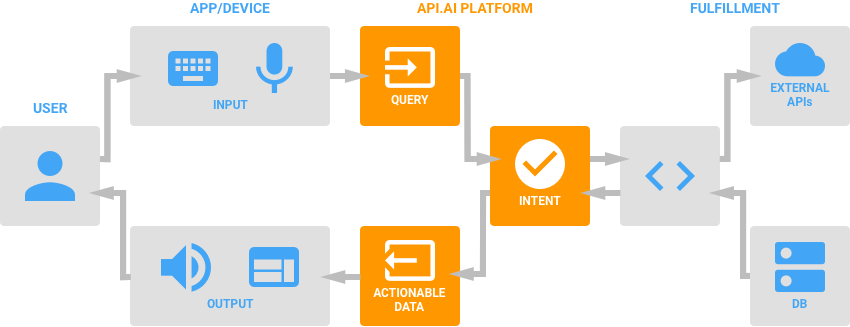
\includegraphics[scale=0.4]{apiai}
		\caption{Architecture of a generic system using \textit{Dialogflow}\cite{apiai}}
	\end{figure}
	
	\section{Fundamental concepts}
		Dialogflow works thanks to some fundamental pillars:
		\begin{itemize}
			\item \textbf{Intents}\\
			They are the mapping between the user query and the desired action. Each intent, indeed, corresponds to "what the user wants to do" in a certain fraction of the conversation.
			\item \textbf{Entities}\\
			They are fragments of natural language inputs, corresponding to a specific type. They can be cities, places, numbers, names, etc. There are a lot of default entities, but custom entities can be created by the user.
			\item \textbf{Actions}\\
			Actions represent what the bot needs to do after the intent has been resolved.
			\item \textbf{Parameters}\\
			They are all the values that are needed to perform an action.
			\item \textbf{Contexts}\\
			They are "containers" in which all the entities and parameters of the conversation are stored. They are fundamental to keep the informations through the conversational flow and make possible the "slot-filling".
		\end{itemize}
	One of the most powerful aspects of \textit{Dialogflow} is the support for slot-filling. It is a technique that lets users to specify details (necessary or not) in different phases of the conversation: this means that the bot can go ahead and keep asking more details to the user before answering the query. Let's make an example:
	
	\begin{verse}
		\textit{Please give me 2 works} - \textbf{User}\\
		\textit{You told me few filters. Do you want to add something?} - \textbf{Bot}\\
		\textit{Yes!} - \textbf{User}\\
		\textit{Ok, tell me what} - \textbf{Bot}\\
		\textit{The artist} - \textbf{User}\\
		\textit{Ok! Just tell me his name} - \textbf{Bot}\\
		\textit{Mozart} - \textbf{User}\\
		\textit{Perfect! Do you want to add something else?} - \textbf{Bot}\\
		...\\
	\end{verse}
	This result is obtained thanks to the "required" entity: in the \textit{Dialogflow} UI (and of course, in the JSON file of the intent) it's possibile to specify some fields that are required for the query to work well. The bot will provide the final answer of the query if and only if all the required slot have been filled! This means that the conversation can go over and over until these informations are provided.\\\\
	The power of \textit{Dialogflow} so, is heavily based on slot-filling. It is able to keep the informations through all the flow of the conversation 

\chapter{The bot}
	\section{The architecture}
	The architecture of the bot is divided in four categories:
	\begin{figure}[H]
		\centering
		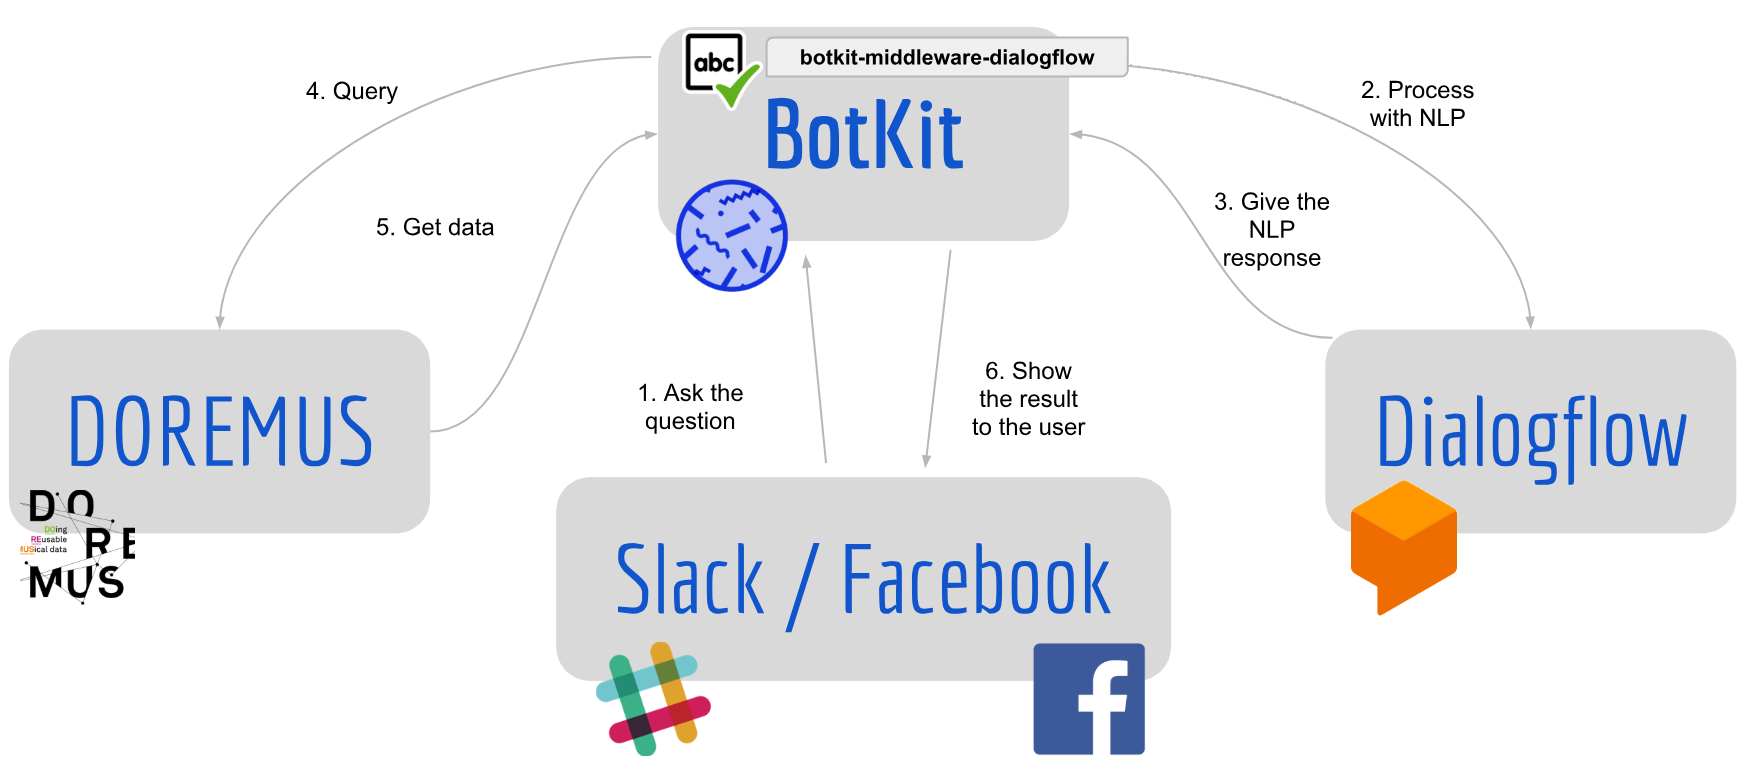
\includegraphics[scale=0.2]{arch2}
		\caption{The high-level architecture of DOREMUS Bot.}
	\end{figure}
	First of all we can find the client, that in the case of our development, testing and validation process, has been \textit{Slack}. Of course, it can be any of the clients which support the installation of the bot on it (\textit{Telegram}, \textit{Facebook Messenger}, etc.). The use of Slack let us to exploit the beautiful \textit{Slack Cards}, to make the answers of our bot (works, artists, performances) prettier and easier to understand in a glance. A set of examples will be provided in the last chapter.\\\\
	The second part of the architecture is represented by the NLP. In this case, as told in the previous chapter, we used \textit{Dialogflow}, to exploit its advanced slot-filling techniques and its NLU power.\\\\
	However, we didn't use \textit{Dialogflow} on its own, exploiting the direct integration with \textit{Slack}, but we used something that we placed in the middle of the two: \textit{Botkit}. \textit{Botkit} is a bot-making toolkit that aims to ease the building process of a bot, potentially exploiting different NLPs and/or different clients. In our case, \textit{Botkit} has been deployed on a web server, and thanks to the \textit{NodeJS} code we were able to come up with a series of features (like the spell checker) that would have been impossible to reach with a simple (direct) integration between \textit{Slack} and \textit{Dialogflow}. We'll talk more about that in the following paragraphs. The communication with the \textit{Dialogflow} NLP is done thanks to a modified version of the \texttt{botkit-middleware-dialogflow}\cite{bmd}: there will be a paragraph dedicated to this middleware in the following pages.\\\\
	The last part of the architecture is of course represented by the data source: \textit{DOREMUS}. We talked about that in the previous chapters, but from the architecture is important to notice how the knowledge graph is queried: each query is dynamic, in the sense that according to the intent, the number of filters and the desired results wanted by the user, the query will have a different shape and a different content. The code in the web server is able to add different pieces of queries according to what \textit{Dialogflow} is able to understand and to provide as output values of the API.\\\\
	The bot code is organized in this way:
	\begin{lstlisting}
	
	bot.js
	spell-checker-middleware.js
	
	config/
		.env
	
	doremus/
		bot_functions.js
	
	slack/
		slack_io.js
		slack_cards.js
	
	facebook/
		facebook_io.js
		facebook_cards.js
		
	dialogflow/
		webhook_server.js
	\end{lstlisting}
	where:
	\begin{itemize}
		\item \texttt{bot.js} is the core file of the bot. It contains the code to declare the fundamental libraries, to start the RTM, and to load the hears methods.
		
		\item \texttt{spell-checker-middleware.js} is the custom module to perform the spell-checking before sending the received sentences to the NLP.
		
		\item \texttt{.env} is the secret file (to place into the \texttt{config} directory) containing all the tokens for \textit{Slack}, \textit{Facebook} and \textit{Botkit Studio}.
		
		\item \texttt{doremus/} contains the files related to the access to the informations of the \textit{DOREMUS} knowledge graph: in this case, contains a single file (\texttt{bot\_functions.js}) that contains all the queries that the bot can do to \textit{DOREMUS}.
		
		\item \texttt{slack/} is a directory containing the files related to \textit{Slack}:
			\begin{itemize}
			\item \texttt{slack\_io.js} contains the methods to receive the sentences sent through \textit{Slack} and processed by the NLU.
			
			\item \texttt{slack\_cards.js} contains the code to build the \textit{Slack} cards to make the answers prettier.
			\end{itemize}
		\item \texttt{facebook/} is a directory containing the files related to \textit{Facebook}:
			\begin{itemize}
			\item \texttt{facebook\_io.js} contains the methods to receive the sentences sent through \textit{Facebook} and processed by the NLU.
			
			\item \texttt{facebook\_cards.js} contains the code to build the \textit{Facebook} cards to make the answers prettier.
			\end{itemize}
		\item \texttt{dialogflow/} is a directory containing the webhook useful for the \textit{Dialogflow} fulfillment phase. This flow is totally detached from our original architecture (which uses \textit{Botkit}), and it's useful only for the lightweight version of the bot which can be used with \textit{Google Home}.
	\end{itemize}
	
	\section{Entities}
	The sentences that the bot is required to recognize are of course full of informations related to the \textit{DOREMUS} knowledge graph. This means that the NLP has to be able to understand some "entities" (informations, words, piece of sentences) that are not in the standard language, but are related to the \textit{DOREMUS} or, in general, musical world. Our bot is equipped with three different entities:
	\begin{itemize}
		\item \texttt{doremus-artist}\\
		Contains all the artists in the \textit{DOREMUS} knowledge graph. It's organized in a \textit{key-value} pair where the \textit{key} is the unique id of the artist inside the knowledge base, and the \textit{value} is the set of full names and surnames of the artist, in all the available language of the knowledge base.
		The query with which the artist were retrieved is the following:
		\begin{lstlisting}

		SELECT DISTINCT ?composer
		  (GROUP_CONCAT (DISTINCT ?name; separator="|") AS ?names)
		  (GROUP_CONCAT (DISTINCT ?surname; separator="|") AS ?surnames)
		  (COUNT (?expression) AS ?count)
		WHERE {
		  ?expression a efrbroo:F22_Self-Contained_Expression .
		  ?expCreation efrbroo:R17_created ?expression ;
		    ecrm:P9_consists_of / ecrm:P14_carried_out_by ?composer .
		  ?composer foaf:name ?name .
		  ?composer foaf:surname ?surname 
		}
		GROUP BY ?composer
		ORDER BY DESC (?count)
		\end{lstlisting}
		The artists are ordered by descending count of works, in order to have the most famous artists at the top of the entity dictionary, and let \textit{Dialogflow} find the most famous artists in case just a surname is given. The result of the query has been taken as a \texttt{.csv} file and then processed a little bit (delete the count, join the names and surnames columns, duplicate the composer id, eliminate the pipes and some special characters) in order to fit with the \textit{Dialogflow}'s constraints.
		
		\item \texttt{doremus-instrument}\\
		Contains all the instruments of the \texttt{iaml/mop/} dictionary of the \textit{DOREMUS} knowledge graph. Also in this case the \textit{key-value} pair dictionary has as keys the id of the instrument, and as values all the synonyms (names in different languages). The query thanks to which we retrieved this entity is:
		\begin{lstlisting}
		
		SELECT DISTINCT ?instr
		  (GROUP_CONCAT (DISTINCT ?instrument; separator="|") AS ?instruments)
		WHERE {
		  ?instr skos:prefLabel ?instrument .
		  ?instr skos:topConceptOf | skos:inScheme ?res .
		  VALUES (?res) {
		    (<http://data.doremus.org/vocabulary/iaml/mop/>)
		  }
		}
		GROUP BY ?instr
		\end{lstlisting}
		
		\item \texttt{doremus-genre}\\
		Contains all the genres of the \texttt{iaml/genre/} dictionary of the \textit{DOREMUS} knowledge graph. The query thanks to which we retrieved this entity is:
		\begin{lstlisting}
		
		SELECT DISTINCT ?gen
		(GROUP_CONCAT (DISTINCT ?genre; separator="|") AS ?genres)
		WHERE {
		  ?gen skos:prefLabel ?genre .
		  ?gen skos:topConceptOf | skos:inScheme ?res .
		  VALUES (?res) {
		    (<http://data.doremus.org/vocabulary/iaml/genre/>)
		  }
		}
		GROUP BY ?gen
		\end{lstlisting}
	\end{itemize}

	\section{Intents}
	The intents are grouped in a simple and clear way, according to what the user wants to retrieve from the \textit{DOREMUS} knowledge graph:
	\begin{itemize}
		\item \texttt{works-by}\\
		Retrieves a set of works according to different filters (artists who composed the works, instruments used, music genre and/or year of composition).
		\item \texttt{find-artist}\\
		Finds a set of artists according to some filters (number of composed works, number of works of a given genre, etc.).
		\item \texttt{find-performance}\\
		Propose to the user a future performance (that can be filtered by city and/or date period), or shows to the user the details of a past performance.
		\item \texttt{discover-artist}\\
		Shows a card with a summary of an artist, with its birth/death place and date, a picture and a little bio. After the card visualization, a set of works of the artist (connection with the \texttt{works-by} intent) can be asked.
	\end{itemize}
	Now we're going to go deeper in the intent descriptions.
	\subsection{Retrieving a set of works}
	The \texttt{works-by} intent is the most complex one in the entire bot's intents set. It can retrieve a certain number of works from 1 to \textit{L}, where \textit{L} is the number specified by the user if it's smaller than the number of available works. Otherwise, if it's greater, all the avilable works are returned. Its default value (if not specified by the user) is 5.\\\\
	The filters can be various:
	\begin{itemize}
		\item \textbf{Artist:}
		the artist name (full or surname).\\
		\textit{"Give me 3 works composed by Bach"}
		
		\item \textbf{Instruments:}
		the instrument(s) (in \texttt{and}/\texttt{or} relation).\\
		\textit{"Give me 2 works for violin, clarinet and piano"}\\
		\textit{"Tell us 4 works for violin or piano"}
		
		\item \textbf{Genre:}
		the music genre.\\
		\textit{"List me 10 works of genre concerto"}
		
		\item \textbf{Composition period:}
		the period in which the work has been written.\\
		\textit{"Tell me one work composed during 1811"}\\
		\textit{"Give us 3 works written between 1782 and 1821"}
		
	\end{itemize}
	The filters can be specified in every way: this means that the user can specify all the available filters, some of them and even none. If the number of filters in the first query is smaller than two, the bot asks the user if he wants to apply other filters. The user can answer positively or negatively, and then decide which kind of filter (and the value) to apply. It's important to notice that the kind of filter and the value can be specified together or not; let's see an example to make it more clear.\\\\
	First of all, we are in the context in which the bot asks the users if he wants to apply some filters:
	
	\begin{verse}
	\textit{Please give me 3 works by Beethoven!} - \textbf{User}\\
	\textit{You told me few filters. Do you want to add something?} - \textbf{Bot}\\
	\textit{Yes!} - \textbf{User}\\
	\textit{Ok, tell me what} - \textbf{Bot}\\
	\end{verse}
	In this case, two scenarios can happen:
	\begin{verse}
	\textit{The composition year} - \textbf{User}\\
	\textit{Of course! Tell me the time period.} - \textbf{Bot}\\
	\textit{Between 1787 and 1812} - \textbf{User}\\
	\end{verse}
	or directly...
	\begin{verse}
	\textit{Only works composed between 1787 and 1812} - \textbf{User}\\
	\end{verse}
	The \textbf{dynamic} query used for the works by artist intent is the following:
	\begin{lstlisting}
	
	SELECT SAMPLE(?title) AS ?title, SAMPLE(?artist) AS ?artist,
	       SAMPLE(?year) AS ?year, SAMPLE(?genre) AS ?genre,
	       SAMPLE(?comment) AS ?comment, SAMPLE(?key) AS ?key
	WHERE {
	
		------------------------------------------------------------ STATIC SECTION
		?expression a efrbroo:F22_Self-Contained_Expression ;
		  rdfs:label ?title ;
		  rdfs:comment ?comment ;
		  mus:U13_has_casting ?casting ;
		  mus:U12_has_genre ?gen .
		?expCreation efrbroo:R17_created ?expression ;
		  ecrm:P4_has_time-span ?ts ;
		  ecrm:P9_consists_of / ecrm:P14_carried_out_by ?composer .
		?composer foaf:name ?artist .
		?gen skos:prefLabel ?genre .
		OPTIONAL {
		  ?ts time:hasEnd / time:inXSDDate ?comp .
		  BIND (year(?comp) AS ?year) .
		  ?expression mus:U11_has_key ?k .
		  ?k skos:prefLabel ?key
		} .
		
		------------------------------------------------------------ DYNAMIC SECTION
		
		------------- Instrument
		?casting mus:U23_has_casting_detail ?castingDetail .
		?castingDetail mus:U2_foresees_use_of_medium_of_performance
		               / skos:exactMatch* ?instrument .
		VALUES(?instrument) {
		  (<http://data.doremus.org/vocabulary/iaml/mop/' <instrument> '>)
		}
		
		------------- Genre
		VALUES(?gen) {
		  (<http://data.doremus.org/vocabulary/iaml/genre/' <genre> '>)
		}
		
		------------- Artist
		VALUES(?composer) {
		  (<http://data.doremus.org/artist/' <artist> '>)
		}
		
		------------- Composition Year
		FILTER (?comp >= "' <yearstart> '"^^xsd:gYear AND
		        ?comp <= "' <yearend> '"^^xsd:gYear)
	}
	GROUP BY ?expression
	ORDER BY rand()
	LIMIT ' <num> '
	\end{lstlisting}
	Some particularities: first of all, the property that let us obtain the instrument:\\ \texttt{mus:U2\_foresees\_use\_of\_medium\_of\_performance
		/ skos:exactMatch*}.\\
	The "\texttt{mus:U2\_foresees\_use\_of\_medium\_of\_performance}" is a property of the \textit{DOREMUS} ontology that allows to connect a generic \textit{castingDetail} to a specific \textit{instrument}. The "\texttt{skos:exactMatch*}" is instead a way to allow the query to search not only in the actual vocabulary used by us (\texttt{iaml/mop/}) but also in other vocabularies that contains an \textit{equivalent} of that instrument. The "\texttt{*}" symbol means \textit{"one or more"}.
	It's also important to notice the particularity of the instrument information because, as previously said, it can be a list of instrument connected by an \texttt{and/or} logic operator. In the query implemented inside the \texttt{works-by} intent, this doesn't mean only to create dynamically the query (like for the other informations) but also to differentiate the code between a single-instrument filter, an "\texttt{and}" multi-instrument filter and an "\texttt{or}" multi-instrument filter. The differences are shown here:
	\begin{lstlisting}
	
	---- AND CASE
	if (strictly === "and") {
	  for (var i = 0; i < instr.length; i++) {
	    query += '?casting mus:U23_has_casting_detail ?castingDetail' + i + ' .
	            ?castingDetail' + i + '
	              mus:U2_foresees_use_of_medium_of_performance
	              / skos:exactMatch* ?instr' + i + ' .
	            VALUES(?instr' + i + ') {
	              (<http://data.doremus.org/vocabulary/iaml/mop/' + instr[i] + '>)
	            }'
	  }
	}
	
	---- OR CASE
	else {
	  query += '?casting mus:U23_has_casting_detail ?castingDetail .
	            ?castingDetail
	              mus:U2_foresees_use_of_medium_of_performance
	              / skos:exactMatch* ?instr .
	            VALUES(?instr) {'
	
	  for (var i = 0; i < instr.length; i++) {
	    query += '(<http://data.doremus.org/vocabulary/iaml/mop/' + instr[i] + '>)'
	  }
	}
	\end{lstlisting}
	In the \texttt{and} case we add (with a \texttt{for} operator that loops through the \texttt{instr} array) a \texttt{castingDetail} for each instrument, forcing its value to that specific instrument. In the \texttt{or} case, instead, the \texttt{castingDetail} is just one and can assume a set of values filled with the \texttt{for} operator that loops through the \texttt{instr} array. 

	\subsection{Finding some artists}
	One powerful intent of the bot is \texttt{find-artist}, that can retrieve a set of artists given some filters. The filters can be for example the birth date or the birth city but the interesting functionality comes thanks to the sorting of the result: having a descending filter, the artists with more works comes first; so, we made the assistant answer questions like:
	\begin{verse}
	\textit{Find the five artists who composed more concerto works} - \textbf{User}\\
	\end{verse}
	or,
	\begin{verse}
	\textit{Find the 3 artists, born between 1752 and 1772, who composed more works} - \textbf{User}\\
	\end{verse}
	or,
	\begin{verse}
	\textit{Find one artist, born between 1752 and 1772, who wrote more works for clarinet} - \textbf{User}\\
	\end{verse}
	and so on.\\\\
	The query of the intent is the following:
	\begin{lstlisting}
	
	SELECT SAMPLE(?name) AS ?name, count(distinct ?expr) AS ?count,
	       SAMPLE(xsd:date(?d_date)) AS ?death_date,
	       SAMPLE(?death_place) AS ?death_place,
	       SAMPLE(xsd:date(?b_date)) AS ?birth_date,
	       SAMPLE(?birth_place) AS ?birth_place
	WHERE {
	  ?composer foaf:name ?name .
	  ?composer schema:deathDate ?d_date .
	  ?composer dbpprop:deathPlace ?d_place .
	  OPTIONAL { ?d_place rdfs:label ?death_place } .
	  ?composer schema:birthDate ?b_date .
	  ?composer dbpprop:birthPlace ?b_place .
	  OPTIONAL { ?b_place rdfs:label ?birth_place } .
	  ?exprCreation efrbroo:R17_created ?expr ;
	    ecrm:P9_consists_of / ecrm:P14_carried_out_by ?composer .
	  ?expr mus:U12_has_genre ?gen ;
	    mus:U13_has_casting ?casting .
	
	  ------------- Genre
	  VALUES(?gen) {
	    (<http://data.doremus.org/vocabulary/iaml/genre/' <genre> '>)
	  } .
		
	  ------------- Instrument
	  ?casting mus:U23_has_casting_detail ?castingDetail .
	  ?castingDetail mus:U2_foresees_use_of_medium_of_performance
	                 / skos:exactMatch* ?instrument .
	  VALUES(?instrument) {
	    (<http://data.doremus.org/vocabulary/iaml/mop/' <instrument> '>)
	  } .
		
	  ------------- Birth date
	  FILTER ( ?b_date >= "' <startdate> '"^^xsd:date AND
	           ?b_date <= "' <enddate> '"^^xsd:date ) .
		
	  ------------- Birth city
	  FILTER ( contains(lcase(str(?birth_place)), "' <city> '") ) .
		
	}
	GROUP BY ?composer
	ORDER BY DESC(?count)
	LIMIT ' <num> '
	\end{lstlisting}
	
	\subsection{Finding some future and past performances}
	The bot is also capable of giving the user some future and past performances and events. The place and the time period can be, of course, specified in the query. The query is the following:
	\begin{lstlisting}
	
	SELECT SAMPLE(?title) AS ?title, SAMPLE(?subtitle) AS ?subtitle,
	       SAMPLE(?actorsName) AS ?actorsName,
	       SAMPLE(?placeName) AS ?placeName, SAMPLE(?date) AS ?date
	WHERE {
	  ?performance a mus:M26_Foreseen_Performance ;
	    ecrm:P102_has_title ?title ;
	    ecrm:P69_has_association_with / mus:U6_foresees_actor ?actors ;
	    mus:U67_has_subtitle ?subtitle ;
	    mus:U7_foresees_place_at / ecrm:P89_falls_within* ?place ;
	    mus:U8_foresees_time_span ?ts .
	  ?place rdfs:label ?placeName .
	  ?actors rdfs:label ?actorsName .
	  ?ts time:hasBeginning / time:inXSDDate ?time ;
 	    rdfs:label ?date .
	  FILTER ( ?time >= "' <startdate> '"^^xsd:date AND
	           ?time <= "' <enddate> '"^^xsd:date ) .
	  FILTER ( contains(lcase(str(?placeName)), "' <city> '") )
	}
	GROUP BY ?performance
	ORDER BY rand()
	LIMIT ' <number> '
	\end{lstlisting}
	It's important to notice the \texttt{ecrm:P89\_falls\_within*} property. It selects not only the place where the event is foreseen, but also the places where that place is contained (so, for example, a city). The "\texttt{*}" means, as usual, \textit{"one or more"}. And here there is an example:
	\begin{verse}
		\textit{Tell me one event in Paris!} - \textbf{User}\\
		\textit{In which period?} - \textbf{Bot}\\
		\textit{Next month} - \textbf{User}\\
	\end{verse}
	\subsection{Know more about an artist}
	The last intent of the bot is \texttt{discover-artist}. This is the richest intent in terms of informations provided: it returns the artist summary in a \textit{Slack card}, with a picture, a short bio, the birth/date places and dates.
	The query is the following:
	\begin{lstlisting}
	
	SELECT ?name, ?bio, ?image,
	       xsd:date(?d_date) AS ?death_date, ?death_place,
	       xsd:date(?b_date) AS ?birth_date, ?birth_place
	WHERE {
	  VALUES(?composer) {(<http://data.doremus.org/artist/' <artist> '>)} .
	  ?composer rdfs:comment ?bio ;
	    foaf:depiction ?image ;
	    schema:deathDate ?d_date ;
	    foaf:name ?name ;
	    dbpprop:deathPlace ?d_place ;
	    schema:birthDate ?b_date ;
	    dbpprop:birthPlace ?b_place .
	  OPTIONAL { ?d_place rdfs:label ?death_place } .
	  OPTIONAL { ?b_place rdfs:label ?birth_place } .
	  FILTER (lang(?bio) = "en")
	}
	\end{lstlisting}
	And here there is an example:
	\begin{verse}
		\textit{Tell me something about Mozart} - \textbf{User}\\
	\end{verse}
	or...
	\begin{verse}
		\textit{What do you know about Beethoven?} - \textbf{User}\\
	\end{verse}
	The bot is also capable of mixing the \texttt{discover-artist} and \texttt{works-by} intents:
	after asking the bot of the details of an artist, the user can retrieve its works, applying the usual filters. Let's make an example:
	
	\begin{verse}
		\textit{Tell me something about Mozart} - \textbf{User}\\
		{[Result with bio, picture, birth/death date/place]}\\
		\textit{Now give me 5 of his works, written for clarinet} - \textbf{User}\\
		{[Result with the 5 works of that artist]}\\
	\end{verse}
	In this case, indeed, the \texttt{works-by} intent is triggered after the \texttt{discover-artist} intent: the artist name, is obtained from the context generated with the \texttt{discover-artist} intent, which is of course still active.

	\section{The spell checker middleware}
	One of the most important aspect of the bot is the misspelling and language detection mechanism, which make it smarter and more reliable. Everything is implemented in an additional middleware located upstream, before the Dialogflow middleware actually send the request to the NLP engine. In this way we intercept every message typed by the user, fixing any typos which otherwise would affect the Dialogflow capabilities to detect intent and entities. In addition we can set the language of the agent, making the bot capable of changing the spoken language at each message. Of course the language detection is a fundamental step in order to use the proper dictionaries during misspelling check.
	
	The core implementation of the middleware could be splitted in 3 parts:
	\begin{enumerate}
		\item Language detection
		\item Misspelling check
		\item Setting of the variables used from the next middleware
	\end{enumerate}
	In the first step we use the \textit{Google Translate API}. For this reason we initially prepare few parameters that we are going to attach to the HTTP request. Among the many, the most important is \texttt{sl} that stands for "source language": setting it to "auto" we let the \textit{Google Translate API} detecting it. This information is in the response JSON.
	
	\begin{lstlisting}[language=C]
	
	// LANGUAGE CHECK
	
	// prepare arguments for the request to Google Translate API
	var url = "https://translate.googleapis.com/translate_a/single"
	var parameters = { 
		q: message.text, 
		dt: 't',
		tl: 'it',
		sl: 'auto',
		client: 'gtx',
		hl: 'it'
	};
	
	request({url:url, qs:parameters}, function(err, response, body) {
	
		if (err) {
			console.log("Error during language detection!");
			next(err);
		}
		
		// get language from json
		var res = JSON.parse(body);
		var lang = res[2];
		
		// update accordingly the speller and the global var 
		if (lang == "fr") {
			speller = spellFR;
			currentLang = "fr";
		}
		else if (lang == "en") {
			speller = spellEN;
			currentLang = "en";
		}
		//otherwise don't change anything
	\end{lstlisting}
	
	In the second step, after setting up the speller accordingly to the language detected, we perform the misspelling check: for each word (splitting by space) we check if is it in the dictionary (in other words well-spelled) otherwise we replace it with the most similar corrected word, if it exists:
	
	\begin{lstlisting}[language=C]
	
	// SPELL CHECKING
	
	// perform the misspelling with the (potentially) updated speller
	var cleanMessage = performMisspellingCheck(message)
	message.text = cleanMessage;
	
	// fill the language field in order to send it to dialogflow api
	message.language = currentLang;
	
	next()
	\end{lstlisting}
	
	The third step is the simplest one: we simply change the text of the message, the object that will handle by the next middleware, with the new, misspelling-free sentence; in addition we set an additional field inside it: the language one, that will be used by \texttt{botkit-middleware-dialogflow} to set the language of the agent before sending the request. This code, differently from the previous one, has to be inserted directly inside the \texttt{botkit-middleware-dialogflow}: after opening a pull-request to the original author, this code was merged into the author's repository.
	
	\begin{lstlisting}[language=C]
	
	if (message.lang) {
		app.lang = message.lang;
	}
	else {
		app.lang = 'en';
	}
	\end{lstlisting}
	
	One minor aspect is behind the variable \texttt{showNewSentence}. We want to give the user a feedback when a correction occurred. When it is set to true, the first next answer will include a warning for the user, indicating the actual sentence that has been processed.
	
	\section{Supported platforms}
	
	\subsection{Textual approach: Slack and Facebook}
	The two supported platforms to communicate with the bot in a textual way are \textit{Slack} and \textit{Facebook Messenger}. Both platforms have been integrated in the \textit{Botkit} environment. The mechanism through which the sentences are heard is simple to understand: the hears methods are instantiated, one for each intent: this methods represent the actions that the bot has to do when an intent is triggered. Usually, without a bot-building environment like \textit{Botkit}, these actions would have been done directly by the "fulfillment" phase in \textit{Dialogflow}. In our case, instead, \textit{Dialogflow} is just an NLP! So, for each platform we use (in this case \textit{Slack} and \textit{Facebook}) we need to instantiate the methods that needs to be triggered when an intent is detected.\\\\
	The prototype of a generic hears functions (in our code) is the following:
	\begin{lstlisting}[language=C]
	
	// HELLO INTENT
	module.exports.hello = botVars.slackController.hears(['hello'], 'direct_message, direct_mention, mention', botVars.dialogflowMiddleware.hears, function(bot, message) {
	
		bot.reply(message, message['fulfillment']['speech']);
	});
	\end{lstlisting}
	The \texttt{hello} variable (put in the module.exports object to be available from the code in other files) is instantiated as an \texttt{hears} (in this case of the \texttt{slackController} object, but it could have been \texttt{fbController}). The code, in the case of the \texttt{hello} intent is really simple, because it just needs to reply with the same answer provided by the \textit{Dialogflow} NLP. For the other intents, the code is obviously more complicated because it needs to get the informations from the \textit{DOREMUS} knowledge graph, as explained in the previous chapters.\\\\
	
	All the textual results that the bot provides are made "prettier" thanks to cards. Both in the \textit{Facebook} and in the \textit{Slack} chat, the results are indeed organized in "key-value" pairs following the JSON syntax. In this way, for example, \textit{Mozart} is presented as the value of the key \textit{Composer}, or \textit{05/12/1791} is the value of the \textit{Death date} key. An example of the code of a card creation is the following:
	\begin{lstlisting}[language=C]
	
	module.exports.getPerformanceCard = function getPerformanceCard(title, subtitle, placeName, actorsName, date) {  
		var performanceAttachment = {
			"type": "template",
			"payload": {
				"template_type": "list",
				"top_element_style": "compact",
				"elements": [
				{
					"title": title,
					"subtitle": subtitle
				},
				{
					"title": "Where",
					"subtitle": placeName
				},
				{
					"title": "When",
					"subtitle": date        
				},
				{
					"title": "Actors",
					"subtitle": actorsName        
				}
				] 
			}
		}
		return performanceAttachment;
	\end{lstlisting}
	
	\subsection{Vocal approach: Google Home}
	The bot supports also a vocal approach for the entire conversational flow. It can reply to the queries with a human voice, like the common vocal assistants. However, in this moment it has some limitations:
	\begin{itemize}
		\item It works only in the english language.
		\item It has a limitation in the artists he knows: 10'000.
		\item It's limited to the \texttt{works-by} and \texttt{find-performance} intents.
	\end{itemize}

	To make it work the \textit{Botkit} architecture has been bypassed: the client communicates directly with the NLP, which understands the query and answers thanks to a webhook (in its fulfillment phase).\\\\
	The webhook has been written by us in NodeJS, to support the \texttt{works-by} and \texttt{find-performance} intents: the bot indeed, replies with a set of works or with a set of scheduled events, basing on the query that has been done.
	
	\section{Logging}
	The bot, during its activity, keeps track of a set of useful informations inside some log files. Each log file is located into the \texttt{/logs} directory and after reaching a given threshold (set at the moment with 1MB), a new file is created: multiple log files can be easier to treat with respect to one huge log file.\\\\
	The logging files have the following structure:
	\begin{itemize}
		\item \texttt{timestamp} - the current date-time.
		\item \texttt{platform} - the platform from which the message comes from (\textit{Slack, Facebook}).
		\item \texttt{user} - the ID of the user sending the message.
		\item \texttt{team} - the team of the user sending the message.
		\item \texttt{intent} - the intent which has been detected by the NLP.
		\item \texttt{confidence} - the confidence level of the NLP in choosing that intent.
		\item \texttt{lang} - the detected language of the message.
		\item \texttt{rawMessage} - the message sent by the user, before spell-checking.
		\item \texttt{cleanMessage} - the message sent by the user, after spell-checking.
		\item \texttt{response} - the answer given by the bot (textual or \texttt{<result\_card>}).
	\end{itemize}
	
	\chapter{Evaluation}
	
	\section{What works}
	The entire path to develop this virtual assistant has been overall successful. The bot knows the artists, the instruments, the genres of the \textit{DOREMUS} knowledge graph, and is capable of answering to a pretty various set of intents.\\\\
	The intents are not just static queries, but the bot engages the user in a tit for tat conversation where the user can specify more filters to the queries it does: this has been done thanks to a smart contexts usage.\\\\
	The bot, indeed, at this phase of its development is able to work with a very large set of queries of medium/high complexity, like the ones listed in the previous chapter; it's fast, the code is stable and overall it provides a pleasant experience also thanks to the visual results it can provide (like artist pictures and cards, in general).\\\\
	It is able (thanks to our custom spell-checker middleware) to correct the major part of common misspellings, which doesn't change too much from the original word.
	
	\section{What can be improved}
	It's also interesting to notice what can improved in the bot. First of all, the non-English languages: in this moment, the bot supports the french language, however \textit{Dialogflow} is not so smart in these languages as it is in English. It needs way more training sentences, which have to combine all possible orderings of entities in the sentences. For example, if the bot is trained on this sentence:
	\begin{verse}
		\textit{"Donne-moi deux oeuvres de Mozart pour clarinet"}
	\end{verse}
	it won't work (if not trained) on these sentences:
	\begin{verse}
		\textit{"Donne-moi deux oeuvres pour clarinet de Mozart"}\\
		\textit{"Dis-moi deux oeuvres pour clarinet de Mozart"}
	\end{verse}
	while in English is a lot smarter and capable to understand also those sentences. It's clear that the ordered combination for all the entities that we can have in a sentence (artists, instruments, genres, numbers, verbs) is huge! So, the bot has to be heavily trained in non-English languages to work well: this can be done also with a script that generates the sentences in all possible order and combination and feeds the bot training pipeline.\\
	Moreover, the \textit{Dialogflow} \texttt{date-period} entity is not fully working in non-english languages, because it's not able to detect expressions like year periods or months. We decided to shut down this filter in the french (and in general, in any of the non-english languages) intents.
	The spell-checking mechanism is not context oriented: this means that the word can be replaced with another one even if the final result is not a totally meaningful sentence. More complex approaches (like RNNs) which take care, after being trained, of the entire context can be used in the future.\\\\
	The \textit{Facebook Messenger} visualization is not so handy for the representation of a big list of informations: this is mainly a platform issue and not a bot one, but it can be ugly when results with a lot of informations have to be showed.\\\\
	There can be some cases (not easy to reproduce, but possible) where the bot can answer in an unexpected way: this is due to the presence of some contexts that are still active after a given flow of sentences. The solution is of course to clear the context, but of course is not a definitive solution and after some phases of the conversation some strange answers could be received when talking to the bot.\\\\
	For what regards entities, a tool that automatically downloads, cleans and updates the bot entities (like FADE\cite{fade}) taking the updated version from the KB can be very useful. It could be put into the \textit{DOREMUS Bot} code to keep fresh all the knowledge that the bot as in the classical music world.\\\\
	With certain queries the bot can be, of course, slow. This is due to the \textit{DOREMUS} knowledge graph and is not under our control: computational-time estimation techniques could be done to say to the user that those queries will take some time to end in a concrete answer.
	
	\chapter{Conclusions}
	
	\begin{thebibliography}{9}
		\bibitem{doremus} DOREMUS: DOing REusable MUSical data. | \textit{\href{http://www.doremus.org/}{http://www.doremus.org/}}
		\bibitem{bobrow} Natural Language Input for a Computer Problem Solving System. 1964. Bobrow, Daniel. | \textit{\href{http://dspace.mit.edu/handle/1721.1/5922}{http://dspace.mit.edu/handle/1721.1/5922}}
		\bibitem{eliza} ELIZA: A computer program for the study of natural language communication between man and machine. 1966. Weizenbaum, Joseph. | \textit{\href{https://dl.acm.org/citation.cfm?id=365168}{https://dl.acm.org/citation.cfm?id=365168}}
		\bibitem{woods} Augmented Transition Networks for Natural Language Analysis. 1969. Woods, William. | \textit{\href{https://eric.ed.gov/?id=ED037733}{https://eric.ed.gov/?id=ED037733}}
		\bibitem{nlpnlunlg} NLP, NLU, NLG and how Chatbots work. | \textit{\href{https://chatbotslife.com/nlp-nlu-nlg-and-how-chatbots-work-dd7861dfc9df}{https://chatbotslife.com/nlp-nlu-nlg-and-how-chatbots-work-dd7861dfc9df}}
		\bibitem{rnn} Attention-Based Recurrent Neural Network Models for Joint Intent Detection and Slot Filling. 2016. Liu, Bing and Lane, Ian. | \textit{\href{https://arxiv.org/abs/1609.01454}{https://arxiv.org/abs/1609.01454}}
		\bibitem{unified} A Unified Architecture for Natural Language Processing: Deep Neural Networks with Multitask Learning. 2008. Collobert, Ronan and Weston, Jason. | \textit{\href{https://ronan.collobert.com/pub/matos/2008\_nlp\_icml.pdf}{https://ronan.collobert.com/pub/matos/2008\_nlp\_icml.pdf}}
		\bibitem{witai} Wit.ai: Turn what your users say into actions. | \textit{\href{https://wit.ai/}{https://wit.ai/}}
		\bibitem{snips} Snips: Using Voice to Make Technology Disappear. | \textit{\href{https://snips.ai/}{https://snips.ai/}}
		\bibitem{watson} IBM Watson: Does your business think? | \textit{\href{https://www.ibm.com/watson/}{https://www.ibm.com/watson/}}
		\bibitem{lex} Amazon Lex: Build conversation bots. | \textit{\href{https://aws.amazon.com/lex/}{https://aws.amazon.com/lex/}}
		\bibitem{luis} Microsoft LUIS: A machine learning-based service to build natural language into apps, bots, and IoT devices. | \textit{\href{https://www.luis.ai/}{https://www.luis.ai/}}
		\bibitem{recast} SAP Recast.ai: A collaborative bot platform. | \textit{\href{https://recast.ai/}{https://recast.ai/}}
		\bibitem{apiai} Chatbots made easy with Dialogflow. An overview on the architecture. | \textit{\href{https://blog.huhtanen.eu/2017/10/15/chatbots-made-easy-dialog-flow.html}{https://blog.huhtanen.eu/2017/10/15/chatbots-made-easy-dialog-flow.html}}
		\bibitem{bmd} The GitHub repository of the Botkit middleware for Dialogflow. | \textit{\href{https://github.com/jschnurr/botkit-middleware-dialogflow}{https://github.com/jschnurr/botkit-middleware-dialogflow}}
		\bibitem{fade} FADE: Filling Automatically Dialog Entities | \textit{\href{https://github.com/marcotrinelli/FADE}{https://github.com/marcotrinelli/FADE}}
	\end{thebibliography}
\end{document}          
